\documentclass[preview]{standalone}
\usepackage{import}
\usepackage{tikz, tkz-euclide}

\begin{document} 
    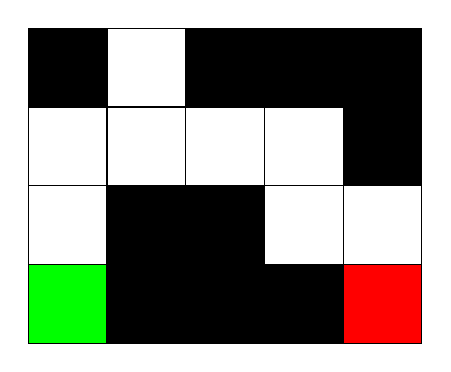
\begin{tikzpicture}
        \begin{scope}[xshift = 3cm, local bounding box = M, block/.style = {minimum size = 1cm, fill = #1, anchor = south west, inner sep = 0pt, behind path}]
            \draw (0, 3) node[block = black]{}
                  (1, 0) node[block = black]{}
                  (1, 1) node[block = black]{}
                  (2, 0) node[block = black]{}
                  (2, 1) node[block = black]{}
                  (2, 3) node[block = black]{}
                  (3, 0) node[block = black]{}
                  (3, 3) node[block = black]{}
                  (4, 2) node[block = black]{}
                  (4, 3) node[block = black]{}
                  (0, 0) node[block = green]{}
                  (4, 0) node[block = red]{}
                  (0, 0) grid (5, 4); 
        \end{scope}
    \end{tikzpicture} 
\end{document}
